Negative numbers and \emph{Subtraction} can be a confusing topic.

Take the time now to learn it well so it does not confuse you later and in the future\footnote{once we start dealing with algebra, quantities will frequently turn negative, and if you cannot understand negative \emph{numbers}, there is little chance you will have a good time with negative \emph{letters}}.

We use the same number line as before, but now instead of \enquote{going forward}, we \enquote{go backwards}.

\begin{figure}[ht]
    \centering
    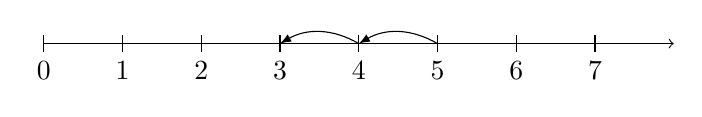
\begin{tikzpicture}
        \draw[->] (0,0) -- (8,0);
        \foreach \x in {0,1,2,3,4,5,6,7}
            \draw[shift={(\x,0)}] (0,3pt) -- (0,-3pt) node[below] {$\x$};
        \foreach \x in {1,2}
            \draw[latex-] (3+\x-1,0) to[bend left] (3+\x,0);
    \end{tikzpicture}
    \caption{the subtraction, $5 - 2 = 3$}
\end{figure}

\begin{examples}
    \begin{questions}
        \Question[3] Carry out these subtractions mentally:
        \begin{multicols}{3}
        \begin{parts}
            \part \(39-31\)=\fillin[7][1cm]
            \part \(27-8\)=\fillin[19][1cm]
            \part \(183-96\)=\fillin[87][1cm]
        \end{parts}
        \end{multicols}
        \Question[2] Now use the Subtraction Algorithm to solve:
        \begin{parts}
            \part \(456-278\)
            \begin{solutionorbox}[1in]
            \end{solutionorbox}
            \part \(20007-7986\)
            \begin{solutionorbox}[1in]
            \end{solutionorbox}
        \end{parts}
    \end{questions}
\end{examples}

\begin{minipage}{\textwidth}
    You should be able to invent the \emph{Subtraction Algorithm}. Think, what are the recipe steps you use when subtracting?\\
    {\large\textbf{Algorithm:}}
    \begin{solutionorbox}[2in]
        Similar to the addition algorithm: you start from right to left and subtract the top most item from the one below it. If you haven't got enough power to subtract the below number from the top, go and borrow 10 units from the next column!
    \end{solutionorbox}
\end{minipage}

\begin{exercises}
    \begin{questions}
        \Question[8] Do these mentally:
        \begin{multicols}{2}
            \begin{parts}
                \part \(28-22\)=\fillin[]
                \part \(273-68\)=\fillin[]
                \part \(350-47\)=\fillin[]
                \part \(94-66\)=\fillin[]
                \part \(137-53\)=\fillin[]
                \part \(167-59\)=\fillin[]
                \part \(475-95\)=\fillin[]
                \part \(1008-17\)=\fillin[]
            \end{parts}
        \end{multicols}
        \Question[6] Do these from left to right:
        \begin{multicols}{2}
            \begin{parts}
                \part \(8+7-7\)=\fillin[]
                \part \(8+12-12-8\)=\fillin[]
                \part \(19-7+8-19\)=\fillin[]
                \part \(56-11+11\)=\fillin[]
                \part \(38-18-1+19\)=\fillin[]
                \part \(101-11+11\)=\fillin[]
            \end{parts}
        \end{multicols}
        \Question[4] Use the algorithm!
        \begin{parts}
            \part \(562-387\)
            \begin{solutionorbox}[1in]
            \end{solutionorbox}
            \part \(921-428\)\\
            \begin{solutionorbox}[1in]
            \end{solutionorbox}
            \part \(405-286\)\\
            \begin{solutionorbox}[1in]
            \end{solutionorbox}
            \part \(813-619\)
            \begin{solutionorbox}[1in]
            \end{solutionorbox}
        \end{parts}
        \Question[6] These are worth double marks.
            \begin{parts}
                \part \(3456-234\)
                    \begin{solutionorbox}[1in]
                    \end{solutionorbox}
                \part \(18502-7862\)
                    \begin{solutionorbox}[1in]
                    \end{solutionorbox}
                \part \(22788-19999\)
                    \begin{solutionorbox}[1in]
                    \end{solutionorbox}
            \end{parts}
        \Question[6] Complete each subtraction by finding a digit for each \(\star\).
        \begin{multicols}{3}
            \begin{parts}
                \part
                    \begin{tabular}{ccc}
                        &7&6\\
                        -&2&$\star$\\
                        \hline\\[-0.4cm]
                        &$\star$&7\\
                        \hline
                    \end{tabular}
                \part
                    \begin{tabular}{ccc}
                        &9&$\star$\\
                        -&$\star$&7\\
                        \hline\\[-0.4cm]
                        &4&6\\
                        \hline
                    \end{tabular}
                \part 
                    \begin{tabular}{ccccc}
                        &2&3&$\star$&$\star$\\
                        -&$\star$&$\star$&9&7\\
                        \hline\\[-0.4cm]
                        &&&3&9\\
                        \hline
                    \end{tabular}
            \end{parts}
        \end{multicols}
        \question Complete each statement by filling in the boxes with numbers that make the statement true.
        \begin{parts}
            \Part[1] \(3+7=10\) is equivalent to \(\square-3=7\)
            \Part[1] \(18+\square=27\) is equivalent to \(\square-18=9\)
            \Part[1] \(42+26=\square\) is equivalent to \(\square-26=42\)
            \Part[1] \(\square+\square=144\) is equivalent to \(144-\square=81\)
        \end{parts}
    \end{questions}
\end{exercises}
